%%%%%%%%%%%%%%%%%
%	Paquetes	%
%%%%%%%%%%%%%%%%%

\documentclass[osajnl,twocolumn,showpacs,superscriptaddress,10pt]{revtex4-1}
%
\usepackage{dcolumn}% Align table columns on decimal point
\usepackage{bm}% bold math
%
%Paquete de Idioma
\usepackage[spanish]{babel}
%
%Codificación Alfabeto
\usepackage[utf8]{inputenc}
%
%Codificación de Fuente
\usepackage[T1]{fontenc}
%
%Índice
\usepackage{makeidx}
%
%Gráficos
\usepackage{graphicx}
\usepackage{subfig}
%\usepackage{xcolor} 
%
%Matemática
\usepackage{amsmath}
\usepackage{amsfonts}
\usepackage{amssymb}
%\usepackage{amstext} 
%
%Estilo de Página Numeración superior
%\pagestyle{headings}
%
%Hiperlinks \href{url}{text}
\usepackage[pdftex]{hyperref}
%
%Graficos y tablas
\usepackage{multirow}
%\usepackage{multicol}
\usepackage{float}
\usepackage{booktabs}
%
\decimalpoint
%\bibliographystyle{IEEEtran}
%\bibliography{IEEEabrv,mybibfile}
%Para tachar dimencionales
\usepackage{cancel}
%
%

%<<<<<<<<< Comando valores absolutos |x| >>>>>
\providecommand{\abs}[1]{\lvert#1\rvert}
%<<<<<<<<< Comando para la normal ||x|| >>>>>
\providecommand{\norm}[1]{\lVert#1\rVert}

%<<<<<<<<< para saltos de página usar  \clearpage >>>>>
%<<<<<<<<< para saltos entre líneas usar \vspace{2cm}>>>>>
%<<<<<<<<< para espaciado horizontal \hspace{1cm}>>>>>
%<<<<<<<<< para colocar url o referencias a url usar \url{http://www.latex-project.org/} o  \href{http://www.latex-project.org/}{latex project}>>>>>>>



%Paquete para configurar medidas de las tablas
\usepackage{tabularx}
%Forma del comando
%\begin{tabular}{|m{0.22\linewidth}|m{0.22\linewidth}|}


%<<<<<<<<< Para configurar \begin{enumerate}[A)]  en donde está la letra "A" escogemos como queremos enumerar, ejemplo \begin{enumerate}[i)]>>>>>>>>>>>>>>
\usepackage{enumerate}

%<<<<<<<<< Cambiar columnas >>>>>
%Se aconseja colocar el documento a una columna y luego cambiarle con forme se vaya utilizando. comandos:
%\begin{multicols}{2}
	%contenido
%\end{multicols}
%\usepackage{multicol} %Paquete cambiar columnas



\begin{document}


%%%%%%%%%%%%%%%%%%%%%%%%%%%%%
%	Autores y filiaciónes	%
%%%%%%%%%%%%%%%%%%%%%%%%%%%%%

%Titulo
\title{Práctica 2: Encendido temporizado con SCR y optoacoplador}
\thanks{Laboratorios de electrónica 4}

\author{Héctor Fernando Carrera Soto, 201700923}\email{e-mail: 3505043180101@ingenieria.usac.edu.gt}
\affiliation{Facultad de Ingeniería, Escuela de ingeniería mecánica eléctrica, Universidad de San Carlos, Edificio T1, Ciudad Universitaria, Zona 12, Guatemala.
}%

%\collaboration{MUSO Collaboration}%\noaffiliation

%\date{\today}%


%%%%%%%%%%%%%%%%%
%	Resumen		%
%%%%%%%%%%%%%%%%%

%\begin{abstract}

    %Un buen resumen debe permitir al lector identificar, en forma rápida y precisa, el contenido básico del trabajo; no debe tener más de 250 palabras y debe redactarse en pasado, exceptuando el último párrafo o frase concluyente. No debe aportar información o conclusión que no está presente en el texto, así como tampoco debe citar referencias bibliográficas. Debe quedar claro el problema que se investiga y el objetivo del mismo.
    
%Para la práctica No.2 de laboratorio se realizó un circuito utilizando como componente principal un optoacoplador, para poder comenzar el aprendizaje respecto a la electrónica de potencia. Para poder comprender su funcionamiento fue necesario realizar un diseño pre establecido con el detalle de cambiarle los parámetros correspondientes que permitieran generar una onda diente de sierra en el osciloscopio virtual. Para ello se realizó un proceso experimental acompañado de los conceptos teóricos aprendidos a través de una investigación, y en dependencia de tales modificaciones, fue posible generar en lugar de una línea recta, una onda diente de sierra.

%\end{abstract}

%%%%%%%%%%%%%%%%%
%	Encabezado	%
%%%%%%%%%%%%%%%%%


\maketitle{}

%%%%%%%%%%%%%%%%%
%	Objetivos	%
%%%%%%%%%%%%%%%%%

\section{Objetivos}

    %Es necesario indicar de manera el propósito del trabajo. Definir los objetivos de la práctica permite la formulación de una o varias hipótesis. Los objetivos se pueden clasificar en objetivos generales y específicos.
    

%                       >>>>>Generales<<<<<<
%\subsection{Generales}

\begin{itemize}
    \item[$\bullet$] Mostrar como un circuito electrónico puede ser utilizado para operar dispositivos eléctricos como motores, relevadores, iluminación, etc.
\end{itemize}

%                       >>>>>Específicos<<<<<<
%\subsection{Específicos}

%\begin{itemize}
    %\item[*] Objetivo específico 1
    %\item[*] Objetivo específico 2
    %\item[*] etc.
%\end{itemize}
 
%%%%%%%%%%%%%%%%%%%%%
%	Marco teórico	%
%%%%%%%%%%%%%%%%%%%%%
 
\section{Marco Teórico}

    %Su contenido debe tener una exposición lógica y ordenada de los temas, así como evitar la excesiva extensión y el resumen extremo de la presentación de la teoría. Es importante que la teoría expuesta no sea una "transcripción bibliográfica" de temas que tengan alguna relación con el problema, sino que fundamente científicamente el trabajo.\\
    
\subsection{Integrado 555}

El circuito integrado 555 es un temporizador eléctrico y se le conoce como “máquina del tiempo” por la gran variedad de tareas que puede realizar con respecto al tiempo. El LM555 tiene internamente una combinación de circuitos digitales y analógicos, se utiliza comúnmente para proporcionar retardos de tiempo, como oscilador a una determinada frecuencia, y como un circuito integrado flip-flop.

\subsection{Conexiones en el integrado}

\begin{itemize}
	\item \textbf{Patilla 1, GND:} Es la patilla de la conexión a Tierra y a ella siempre se conecta la masa o el negativo de la pila (0V = cero voltios).
	
	\item \textbf{Patilla 2, Trigger:} Es la parte del circuito integrado donde se establece el inicio del tiempo de retardo para la configuración monoestable del LM555. Para que ocurra este proceso el pulso disparador disminuye el voltaje (1/3)Vcc, donde Vcc corresponde al voltaje de alimentación.
	
	\item \textbf{Patilla 3, OUT:} En este pin se puede observar el resultado de la configuración del temporizador eléctrico ya sea como monoestable, estable u otra opción.
	
	\item \textbf{Patilla 4, Reset:} Para un nivel de voltaje por debajo de 0.7 V, tiene la función de poner el pin de salida a nivel bajo. Para evitar el reinicio se deberá conectar este pin a alimentación.
	
	\item \textbf{Patilla 5, Control:} Al utilizar el circuito integrado LM555 como controlador de voltaje, el voltaje en esta terminal puede variar teóricamente desde Vcc hasta aproximadamente 0 V, en la práctica la variación es de Vcc – 1.7 V hasta casi 2 V menos.
	
	\item \textbf{Patilla 6, Umbral (Threshold):} Corresponde a la entrada de un comparador interno de umbral el cual se emplea para poner la señal de salida a un nivel bajo.
	
	\item \textbf{Patilla 7, Descarga (Dis):} Permite descargar el condensador externo al circuito integrado 555 para su funcionamiento.
	
	\item \textbf{Patilla 8, Vcc:} Es el pin donde se conecta el voltaje o tensión de alimentación que va de 4.5 voltios hasta 16 voltios (máximo).
\end{itemize}

\subsection{Circuito Multivibrador Monoestable con 555}

Se denomina monoestable a un circuito que permanece estable en un solo estado. “El circuito 555 configurado como monoestable entrega a su salida un solo pulso de ancho establecido por el diseñador del circuito. La señal de disparo (trigger) debe ser de nivel bajo y de muy corta duración.

\begin{figure}[H]
\centering
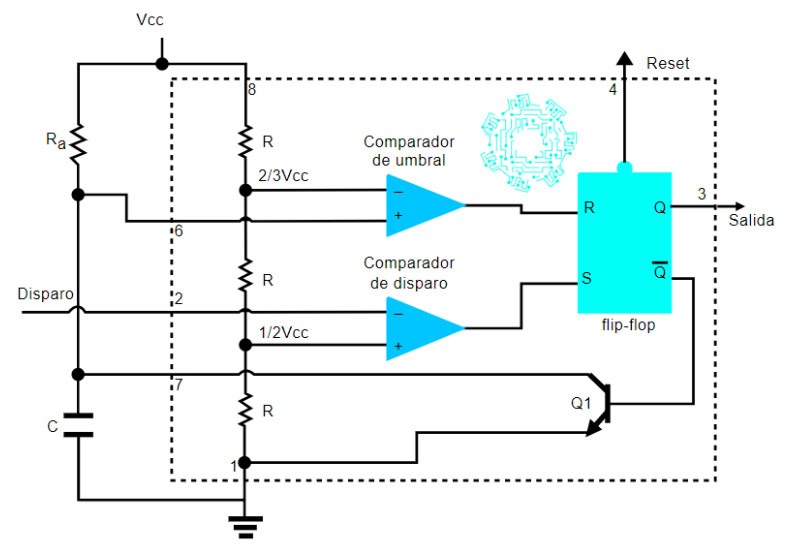
\includegraphics[width = \columnwidth]{Fig_1.png}
\caption{Configuracion interna del 555 Monoestable
Fuente: Elaboración propia.}
\end{figure}

\subsubsection{Datos del circuito después del disparo}

Al presionar el interruptor de disparo del circuito, el voltaje en el pin 2 del 555 baja bruscamente, activando el temporizador. Para que este disparo sea válido, el voltaje aplicado al pin 2 debe ser menor a $\frac{1}{3}$ V+.

\begin{figure}[H]
\centering
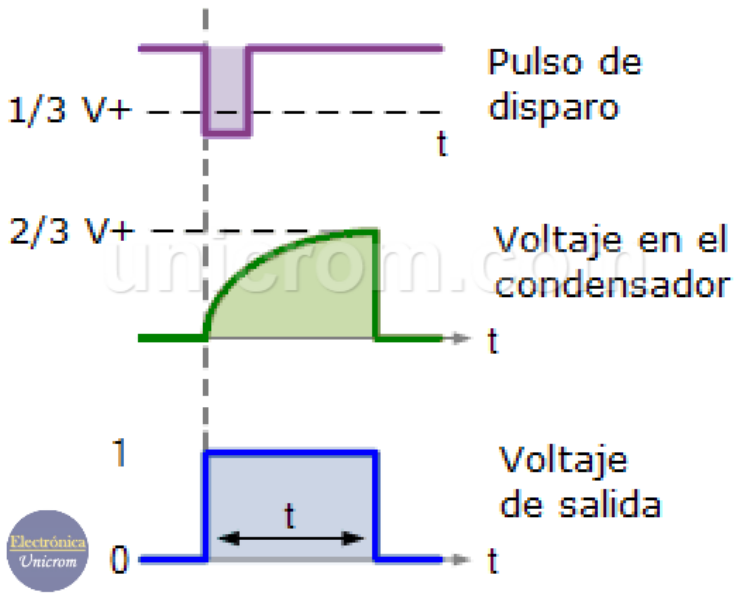
\includegraphics[width = \columnwidth]{Fig_2.png}
\caption{}
\end{figure}

El condensador, que estaba totalmente cargado, se descarga bruscamente y tiene entre sus terminales 0 V. El condensador ahora empieza el proceso de carga hasta que el voltaje en sus terminales llegue a ser 2/3 V+. En el momento en que esto ocurre el voltaje regresa nuevamente a 0V.\\

El voltaje de salida que inicialmente estaba en 0 V sube bruscamente a V+ en el momento en que se aplica el pulso de Disparo y se mantiene en este nivel hasta que el condensador se haya cargado a2/3V+, como se menciona en el párrafo anterior.\\

El tiempo que la salida está en nivel alto depende de la siguiente fórmula:\\

\begin{equation}
T = 1.1 * R_{1} * C_{1} \ [s]
\end{equation}

\subsection{MOC3021}

El MOC3021 es un optoacoplador, también llamado
optoaislador, un dispositivo de emisión y recepción que funciona como un interruptor activado mediante la luz emitida por un diodo LED, que satura un componente opto electrónico.\\

\begin{figure}[H]
\centering
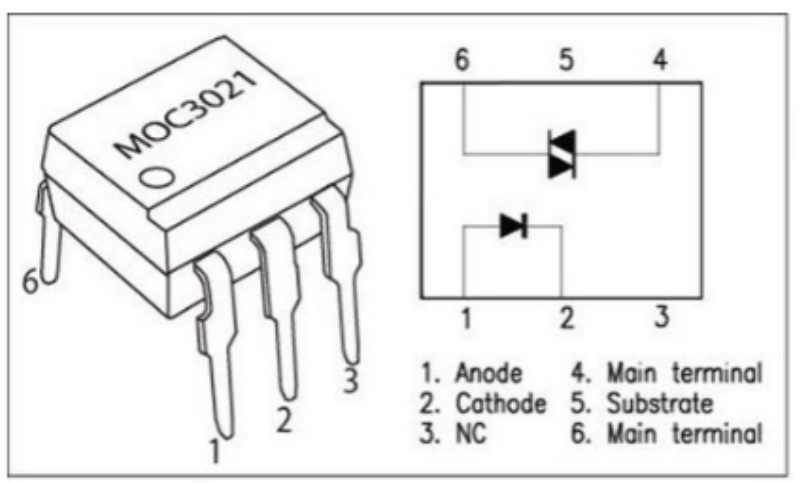
\includegraphics[width = \columnwidth]{Fig_3.png}
\caption{Diagrama de un MOC3021.}
\end{figure}

%%%%%%%%%%%%%%%%%%%%%%%%%%%%%
%	Diseño experimental		%
%%%%%%%%%%%%%%%%%%%%%%%%%%%%%

\section{Diseño Experimental}

    %Hace una descripción del método o técnica utilizada para medir y/o calcular las magnitudes físicas en estudio, y si es del caso, del aparato de medición. Hay que recordar que el "método" es el procedimiento o dirección que conducirá a la solución del problema planteado. Se recomienda redactar una breve introducción para explicar el enfoque metodológico seleccionado.\\
    



\subsection{Cálculos realizados}

En esta practica se que el circuito Monoestable multivibrador, tuviese un tiempo de 5 segundo, por lo cual, se hizo el cálculo necesarios para encontrar la resistencia adecuada para este tiempo. En donde se hizo el despeje de la ecuación No.1 para este calculo.\\

Dónde:\\
$C_{1} = \ 100 \ \mu F$\\
$T = 5 \textup{s}$\\

Por lo que procedemos al despeje de la Ecuación.\\

\begin{align*}
T &= 1.1 * R_{1} * C_{1}\\
R_{1} &= \dfrac{T}{1.1 * C_{1}}
\end{align*}

Sustituimos valores:\\

\begin{align*}
R_{1} &= \dfrac{5 \ s}{1.1 * 100 \ \mu F}\\
R_{1} &= 45.45 \ k \Omega
\end{align*}


%%%%%%%%%%%%%%%%%
%	Mateiales	%
%%%%%%%%%%%%%%%%%

%\subsection{Materiales}

%\begin{itemize}
    %\item[*] Material 1
    %\item[*] Material 2
    %\item[*] etc.
%\end{itemize}

%%%%%%%%%%%%%%%%%%%%%%%%%%%%%%%%%%%%%
%	Magnitudes físicas a medir		%
%%%%%%%%%%%%%%%%%%%%%%%%%%%%%%%%%%%%%

%\subsection{Magnitudes físicas a medir}

%\begin{itemize}
    %\item[*] Magnitud física a medir 1
    %\item[*] Magnitud física a medir 2
    %\item[*] etc.
%\end{itemize}

%%%%%%%%%%%%%%%%%%%%%
%	Procedimiento	%
%%%%%%%%%%%%%%%%%%%%%

%\subsection{Procedimiento}

%\begin{enumerate}
    %\item[*] Procedimiento 1
    %\item[*] Procedimiento 2
    %\item[*] etc.
%\end{enumerate}

%%%%%%%%%%%%%%%%%
%	Resultados	%
%%%%%%%%%%%%%%%%%

\section{Resultados}

    %Los resultados se analizan, en general, por medio de gráficos o diagramas, debidamente identificados, que muestran el comportamiento entre las magnitudes medidas o que permiten calcular otras magnitudes. Dependiendo de lo extenso de las gráficas y/o tablas, éstas se pueden anexar al final del trabajo.\\
   
    %Todos los datos obtenidos deben ir acompañados de las unidades dimensionales, con su debida incertidumbre de medida, que mostrarán la calidad, precisión y reproductibilidad de las mediciones. Éstos deben ser consistentes, a lo largo del reporte.\\
    
\begin{itemize}
	\item Se procedio a la contruccion de los circuitos en el Simulador de circuitos Proteus 8, tal y como se muestra en las siguientes Figura:
\end{itemize}

\begin{figure}[H]
\centering
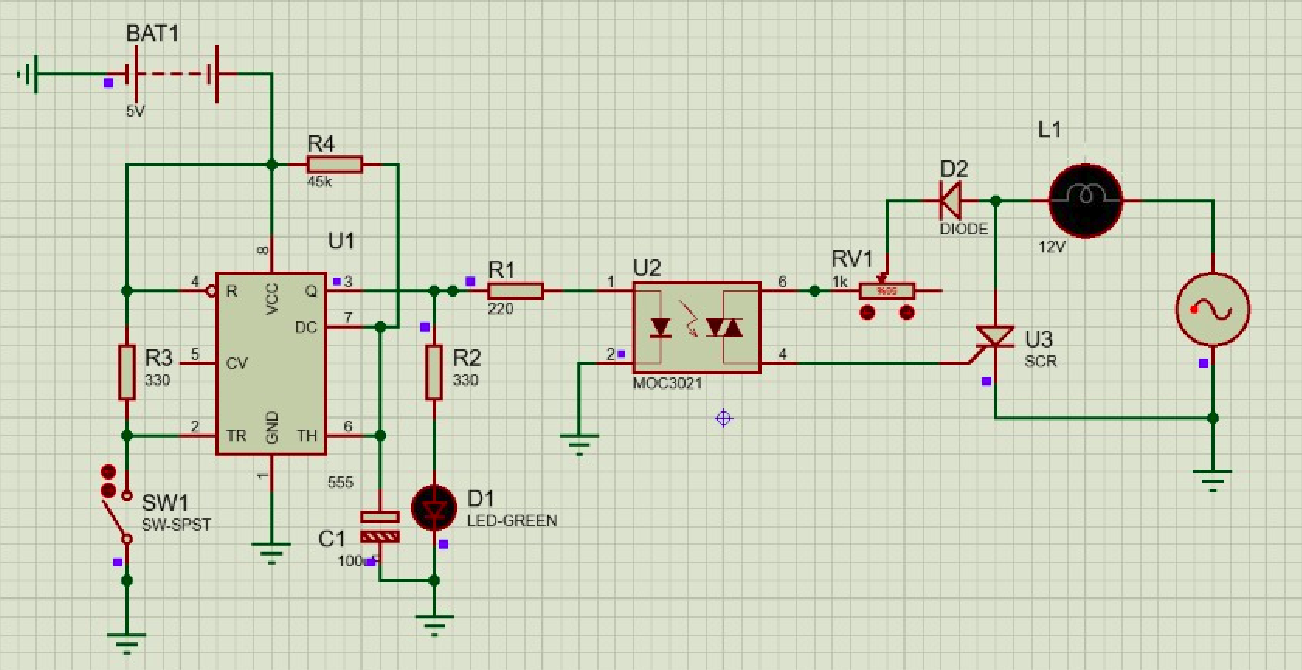
\includegraphics[width = \columnwidth]{Fig_4.png}
\caption{Circuito 1 con Swich}
\centering{Fuente: Elaboración propia.}
\end{figure}

\begin{figure}[H]
\centering
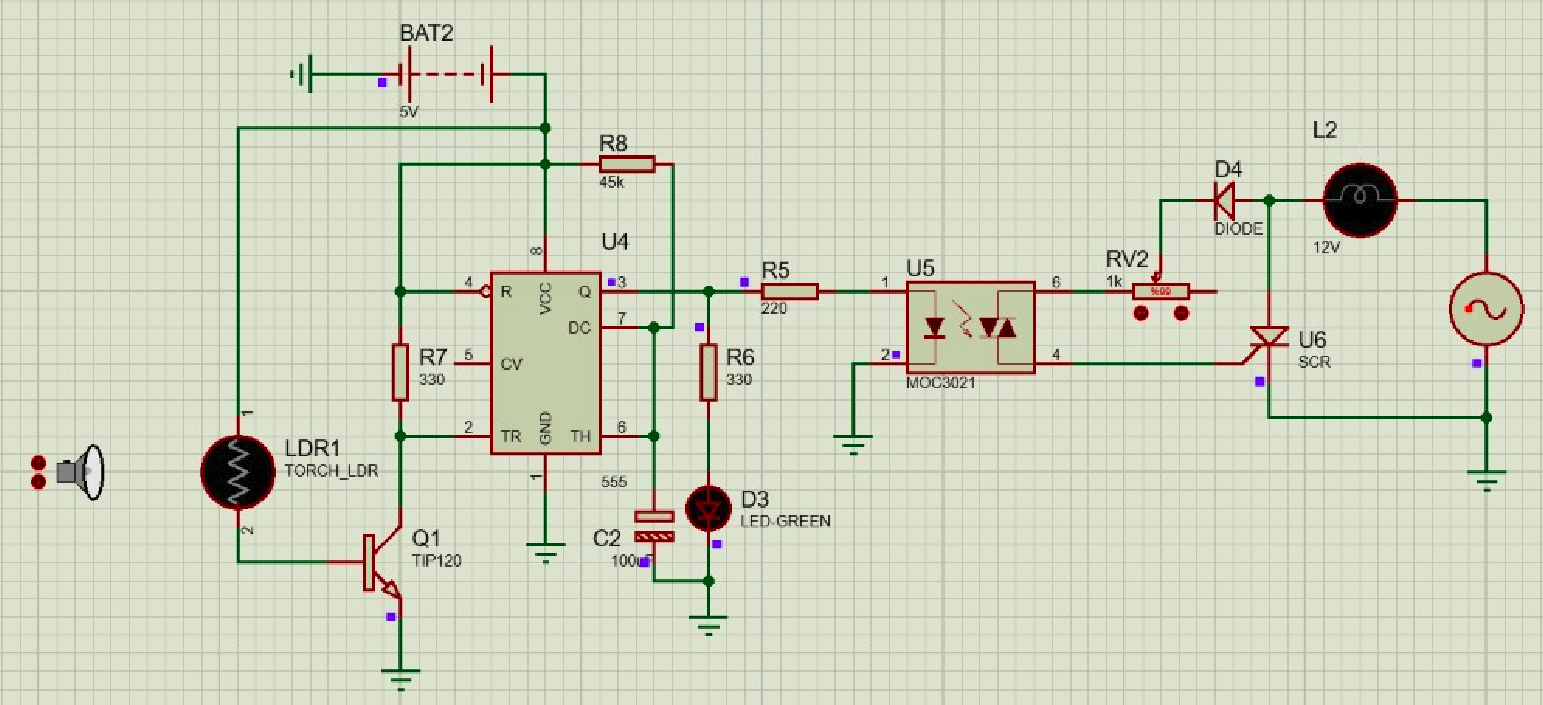
\includegraphics[width = \columnwidth]{Fig_5.png}
\caption{Circuito 2 con LDR}
\centering{Fuente: Elaboración propia.}
\end{figure}
%%%%%%%%%%%%%%%%%%%%%%%%%%%%%%%%%
%	Discusión de resultados		%
%%%%%%%%%%%%%%%%%%%%%%%%%%%%%%%%%

\section{Discusión de Resultados}

    %En este apartado se deben analizar los resultados obtenidos, contrastándolos con la teoría expuesta en la sección del Marco Teórico. Corresponde explicar el comportamiento de las tablas y gráficas expuestas en la sección de Resultados, tomando en cuenta el análisis estadístico apropiado.\\
    
\begin{itemize}
	\item Al analizar el circuito se observa que si se mantiene preciondado el swich el circuito no se activa, esto debido a que en este momento el circuito tiene un voltaje mucho mayor al 1/3 de Vcc, pero al quitar el swich se activa el circuito, ya que el voltaje, $q$, entra en el comparador del 555 es mejor, por lo tanto activa el circuito.
 
	\item Al usar el sendor LDR se observa que al, activarlo mediante luz, el circuito no hace nada, pero al quitar la luz, el sensor se enciende, esto debido a que funciona similar, a cuando usamos un swich.
\end{itemize}

%%%%%%%%%%%%%%%%%%%%%
%	Conclusiones	%
%%%%%%%%%%%%%%%%%%%%%

\section{Conclusiones}

    %Las conclusiones son interpretaciones lógicas del análisis de resultados, que deben ser consistentes con los objetivos presentados previamente.\\

\begin{enumerate}
    \item El tiempo de encendido dependerá de la resistencia de descarga del capacitor. el cual a su vez activara el MOC3021 y se encendera la lampara.\\
    
    \item Al tener un voltaje de menor a 0.7 en el reset del integrado 555, cuando presionamos el swich este no se activa, pero al desactivarlo, este lleva a un voltaje mayor, y a su vez, el voltaje en el Trigger, es menor a 1.33 lo cual hace que ese active el circuito.\\
    
    \item Se debe verificar bien las discrepancias del simulador, dado que hay algunos simuladores que tienen variaciones en los datos conforme a la simulación.
\end{enumerate}


%%%%%%%%%%%%%%%%%%%%%
%	Bibliografías	%
%%%%%%%%%%%%%%%%%%%%%


\begin{thebibliography}{99}
%Las fuentes de consulta se citan en forma organizada y homogénea, tanto de los libros, de los artículos y, en general, de las obras consultadas, que fueron indispensables indicar o referir en el contenido del trabajo.

\bibitem{} BOYLESTAD, ROBERT L. y NASHELSKY, LOUIS
(2009) \textit{Electrónica: Teória de Circuitos y Dispositivos
Electrónicos}

\bibitem{} J.A. Gualda, S. Martínez, P.M. Martínez (2001) \textit{Electrónica Industrial: Técnicas de Potencia}

\end{thebibliography}

\end{document}
